

\section{Theory on the LPM and Windowing: OE Setup}\label{se:theoryLPMandWindowing}

Details of the theory pertaining to this section may be found in \cite{schoukens2010nonparametric}, basic aspects of which are presented below.

\subsection{Spectral Nonparametric Model and Assumptions}

Using convolution, the noiseless output signal in Fig. \ref{lpmtdrep} is $y_0(t) = g_0(t)*u_0(t)$, where the signals are sampled at $t = 0, 1, 2,...,N-1$ and the excitation signal $u_0(t)$ is random noise. As shown in \cite{FDidentEd2Pintelon} and \cite{Pintelon1997} the DFT spectra of the sampled signals at the frequency $\Omega_k$ are related as follows:
\begin{equation}\label{lpmleak}
Y_0(k)=G_0(\Omega_k)U_0(k)+T_G(\Omega_k)
\end{equation}
where $U_0(k)$ is the DFT spectrum of the random noise excitation,  $G_0(\Omega_k)$ is the transfer function and $T_G(\Omega_k)$ is the transients leakage term. 
In this paper, the DFT of a signal $x(t)$ is defined explicitly as  \cite{Oppenheim1983}

\begin{equation}\label{eq:defDFT}
X(\Omega_k) = \frac{1}{\sqrt{N}}\sum_{t=0}^{N-1}x(t)e^{-\frac{j2\pi kt}{N}}
\end{equation}

The following assumptions are consistent with \cite{schoukens2010nonparametric} for an OE setup (Fig. \ref{lpmtdrep}):
\begin{assumption}
The SISO system $G_0$ and  the transients leakage spectrum $T_G$ are both smooth functions of the frequency.
\end{assumption}

\begin{assumption}

The spectrum of the  input signal $U_0$ is not a smooth function of the frequency, but a rough function, for example $U_0(k+1) - U_0(k)$ should not vanish to zero. %i.e. $U_0(k+1) - U_0(k) \neq 0$. 
\end{assumption}

In other words, for the excitation signal to be rough: the magnitude of the spectral difference $|U_0(k+1) - U_0(k)|$ must have a probability of 1 (unity) for it to remain in the same order of magnitude as $|U_0(k)|$, irrespective of the record length $N\rightarrow\infty$ and the corresponding  frequency resolution $f_0\rightarrow{0}$.

\begin{assumption}
The measured output signal is $y(t) = y_0(t) + v(t)$ with the exact input signal $u_0(t)$ known. 
\end{assumption}

\begin{assumption}
The filtered white noise $v(t) = H_0(q)e(t)$ is the disturbing noise source at the output.
\end{assumption}

\subsection{The Hanning Window and the LPM}\label{se:LPMFRFest}%\label{se:FRFhanningLPM}
\subsubsection{Windowing}
The effect of windowing may be  exemplified by use of the Hanning window, which is very popular.  In a nutshell, the Hanning window is effective in reducing  the leakage errors, but  with a trade off of increased interpolation errors. %This is because the term $G_0(\Omega_k)U_0(k)$ in equation \eqref{lpmtd1} is not smooth and $G_0(\Omega_k)$ varies with the frequency. 
Pertinent details of the Hanning window are discussed in \cite{schoukens2006leakagereduction,Antoni20071723,schoukens2010nonparametric,Wellstead198155} and \cite{harris1978}.

The anomalies due to interpolation errors, associated with windowing, can easily be mitigated or circumvented by use of the LPM. As shown in \cite{FDidentEd2Pintelon}, the leakage errors are reduced from  $\mathcal{O}({N}^{-1})$, for Hanning windowing, to $\mathcal{O}({N}^{-3})$ or better, for the LPM.

\subsubsection{Formulation of the Linear LS LPM}
The LPM is formulated as a nonparametric local-linear-least-squares (LS) estimate using the full data record of length \emph{N} as outlined below \cite{schoukens2010nonparametric}. Section 7.2.2 of \cite{FDidentEd2Pintelon} 
gives the general formulation of the LPM for MIMO systems. The formulation in this paper is a summary for a SISO system.

The DFT spectra at the output of the SISO system in Fig. \ref{lpmtdrep} are derived from equations \eqref{lpmtd1} and \eqref{lpmleak}, \emph{viz}:
\begin{equation}\label{lpm1spectra}
Y(k)=G_0(\Omega_k)U_0(k)+T(\Omega_k)+V_0(k)
\end{equation}
where $V_0(k) = H_0(\Omega_k)E(k)$ is a noise term, and $T(\Omega_k)$ is the leakage term. The latter is the sum of the system and the noise leakage terms, i.e. $T(\Omega_k) = T_G(\Omega_k) + T_H(\Omega_k)$.

The smooth characteristics of $G_0(\Omega_k)$ and $T(\Omega_k)$ allow for the use of the Taylor series representations at the frequency lines $k+r$ in a frequency domain window of width $2n+1$, with a remainder $\mathcal{O}\left(\frac{r}{N}\right)^{(R+1)}$ of the first order Taylor series expansion \cite{schoukens2010nonparametric}, \emph{viz}:
\begin{align}\label{lpmGTaylorS}
G_0(\Omega_{k+r})&=G_0(\Omega_k)+\sum_{p=1}^{R}g_p(k)r^p+\mathcal{O}\left(\frac{r}{N}\right)^{(R+1)},
\\
\label{lpmTTaylorS}
T(\Omega_{k+r})&=T(\Omega_k)+\sum_{p=1}^{R}t_p(k)r^p+N^{-1/2}\mathcal{O}\left(\frac{r}{N}\right)^{(R+1)},
\\
\text{where}&\ r\in\mathbb{W}_n,\quad \mathbb{W}_n = \{-n,-n+1,\dots,n\}
\end{align}

The choice of the tunable parameters $n$ and $R$ is discussed later on.

Neglecting the remainder, the Taylor series approximation of \eqref{lpm1spectra} can be written in a matrix vector form, \emph{viz}:
\begin{equation}\label{lpmGTMatrix}
Y(k+r)\approx{K(k, r)\theta(k)+V_0(k+r)}
\end{equation}
where $\theta(k)\in\mathbb{C}^{2R+2}$ is the column vector of the  parameters ($G_0(\Omega_k)$, $T(\Omega_k)$, $g_p$, $t_p$, and $p = 1, 2, ...., R$) and $K(k, r)$ is the row vector of their respective coefficients:
\begin{align}
K(k,r) = &\left[
\begin{matrix}
U_0(k+r) & U_0(k+r)r & \dots 
\end{matrix}
\right.
\\ 
&\quad\left.\begin{matrix}U_0(k+r)r^R & 1& r&\dots&r^R\end{matrix}\right]\nonumber
\end{align}

Equation \eqref{lpmGTMatrix} can be written in the more compact (stacked vectors) form:
\begin{equation}\label{lpmGTMatrixStack}
Y_n(k)\approx K_n(k)\theta(k)+V_n(k)
\end{equation}
where $Y_n(k), V_n(k)\in\mathbb{C}^{2n+1}$, and $K_n(k)\in\mathbb{C}^{(2n+1)\times(2R+2)}$ are the stacked values of $Y(k+r)$, $K(k,r)$, and $V_0(k+r)$, respectively, for $r\in\mathbb{W}_n$.
The estimates of the parameters $\theta(k)$ are obtained as the minimizers of the least squares problem, \emph{viz}:
\begin{align}\label{eq:LSsolutionLPM}
\hat\theta(k) = \argmin_{\theta(k)} \left\|Y_n(k) - K_n(k)\theta(k)\right\|_2^2
\end{align}

The formulation of

 equation \eqref{eq:LSsolutionLPM} must take into account the fact that  a full rank of $K_n$ requires $n \geq R + 1$. The choice $n = R + 1$ results in the highest variance on the estimate, but with the smallest interpolation error \cite{schoukens2010nonparametric}. %(per JL)!

The values $R = 2$, and $n=R+1=3$ will be used in the LPM.

When substituted into equations \eqref{lpmGTaylorS} and \eqref{lpmGTMatrix},
 these yield the following quadratic local polynomials of $G_0$ and $T$ around a central frequency $\Omega_{k}$:
\begin{align}\label{lpmImplQuadG}
G_0(\Omega_{k+r})&\approx G_0(\Omega_k)+g_1r+g_2r^2
\\
T(\Omega_{k+r})&\approx T(\Omega_k)+t_1r+t_2r^2\label{lpmImplQuadT}
\end{align}

\noindent
($r\in\mathbb{W}_3$)
and the vector of parameters:

\begin{equation}\label{lpmThetaEst}
\theta^\top(k)=\left[G_0(\Omega_k) \ g_1 \ g_2\  T_G(k)\  t_1 \ t_2\right]
\end{equation}
The LPM estimate of the FRF is the first element of the estimate $\hat\theta(k)$, obtained from \eqref{eq:LSsolutionLPM}, \emph{viz}:

\begin{equation}
\hat{G}_\text{poly}(\Omega_k) = \hat\theta_1(k)
\end{equation}

The estimation of $\hat{G}_\text{poly}(\Omega_k)$ at a single frequency $\Omega_k = 0.586$~Hz is illustrated in Fig. \ref{LPM_Schematic_EG}.% centered at $k$, where $r = 0$.
\begin{figure}[htb] %  figure placement: here, top, bottom, or page
   \centering

   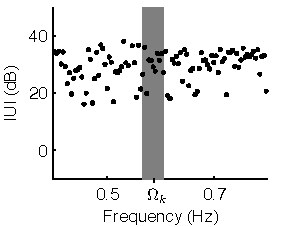
\includegraphics[scale=0.92]{spectUOmegak} 
   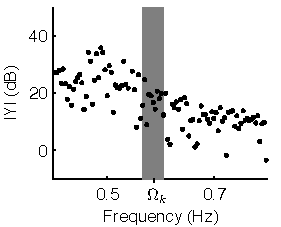
\includegraphics[scale=0.92]{spectYOmegak} 
   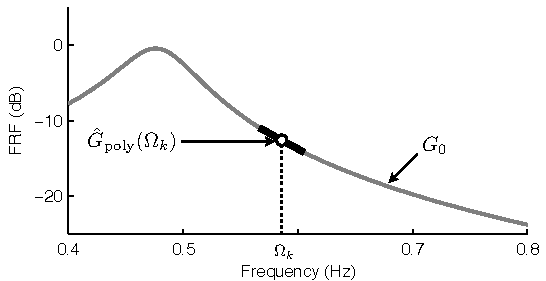
\includegraphics{LPMfigOmegak} 
   \caption{Illustration of the LPM. Top figures: input spectrum (left) and output spectrum (right). A small band is selected (gray area, top figure), in which $\hat G_\mathrm{poly}(\Omega_{k+r})$ is estimated (black thick line, bottom figure) as a local polynomial. Only its central value $\hat G_\mathrm{poly}(\Omega_k)$ (white circle) is retained. This procedure is repeated for all $\Omega_k$.}

   \label{LPM_Schematic_EG}
\end{figure}
This procedure is repeated at each central frequency $\Omega_k$ for  $k\in \{1,\dots,N/2\}$ (i.e. the entire frequency band, including Nyquist, but excluding DC, and regularizing at the boundaries). This completes the LPM, yielding an intrinsic averaging of the spectra of the estimated FRF, $\hat{G}_\text{poly}(\Omega_k)$.

